\documentclass{article}
\usepackage{amsmath,amssymb,setspace,verbatim,graphicx,enumerate,enumitem}
\usepackage[top=1in,bottom=1in,left=1in,right=1in,head=0.5in,foot=0.5in]{geometry}
\usepackage{caption}
\usepackage{mathtools}
% \usepackage{subcaption}
% \usepackage{subfig}
% \usepackage{subfloat}
% \usepackage{tabularx}
\usepackage{mdframed}
\usepackage{amsthm}

\newtheorem*{theorem}{Theorem}

\newenvironment{Rcode}% environment name 
{%begin code
    \begin{mdframed}
    \#R code
    \begin{small}
}
{%end code
    \end{small}
    \end{mdframed}
}

\newenvironment{console}% environment name 
{%begin code
    \begin{mdframed}
    \#Console
    \begin{small}
}
{%end code
    \end{small}
    \end{mdframed}
}

\begin{document}
\title{STDA Homework 1}
\author{Seokjun Choi}
\date{April 10, 2020}
\maketitle

Note: \\
You can get full, run-able code files at my github page: Visit https://github.com/letsjdosth/SpaTempoDA \\
Because I provide the full code file separately, in this report 
I will show key-code blocks only instead of bringing the full, verbose code.

\section{Problem 1}
\textbf{
Suppose we want to simulate a random vector $Y \sim N(\mu, \Sigma)$.
If $\Sigma$ (Matern) is symmetric and positive definite, it can be represented using the
Cholesky decomposition $\Sigma = LL'$, where $L$ is a lower triangular matrix.
Consider the following algorithm for simulating Y:
\begin{itemize}
    \item Calculate the matrix $L$.
    \item Sample $Z \sim N(0,I)$, where $I$ is the $n \times n$ identity matrix.
    \item Let $Y=\mu+LZ$
\end{itemize}
}
\subsection{Problem 1-(a)}
\textbf{
Show that $Y$ generated in this way has the correct distribution.
You may use the fact that a linear function of a multivariate normal random variable is
again multivariate normal; just show the mean and variance are correct.
}

From the elementary observation from mathematical statistics, we have
for $a,b \in \mathcal{R}$ and for a random variable $X$,
\[E[aX+b] = aE[X]+b\]
\[Var[aX+b]=a^2 Var[X]\]
And its multivariate version is, for proper $A\in\mathcal{R}^{n\times n}$, $b\in\mathcal{R}^n$,
and for a random vector $X$,
\[E[Ax+b]=AE[X]+b\]
\[Var[AX+b]=AVar[X]A'\]
Then, using this observation and the fact at this problem, we can get
\[Y \sim N(\mu + 0, LIL')\]
Since $LL'=\Sigma$ by our setting, we get \(Y \sim N(\mu, \Sigma)\), so we can confirm that the algorithm is valid.



\subsection{Problem 1-(b)}
\textbf{
Write a function or a few lines of code in R to implement this method
for arguments mu and Sigma. You may use the built-in function chol for the Cholesky decomposition and rnorm to generate Z.
}

Here is implementation of the key part.

\begin{Rcode}
    \begin{verbatim}
rnorm_chol_algorithm = function(mu, Sigma) {
    # mu is vector
    # Sigma should be symmetric, positive definite matrix
    dimension = dim(Sigma)
    vecZ = rnorm(dimension, 0, 1)
    chol_upperL = chol(Sigma)
    return(mu + t(chol_upperL) %*% vecZ)    
}
    \end{verbatim}
\end{Rcode}



\subsection{Problem 1-(c)}
\textbf{
For a mean and covariance function of your choosing, use your code from (b) and
make a few plots illustrating realizations of a Gaussian process on [0;1], but changing the different parameters in the model.
These differences will be easier to see if you keep the same Z sample but just change mu and Sigma.
}

For convenience, I use fields\$Matern function to calculate covariance matrix from parameters of Matern.
And for easy visualization, I will make only 2 dimensional chain.
Here are 3 test cases. (In full code, there is one more case for ordinary(not Matern) GP, but you may ignore it.)

Fix $\rho$ to 1. And,
\begin{itemize}
    \item $\nu = 0.1$ (in code, test 3)
    The covariance matrix becomes
    \[\begin{bmatrix}
        1 & 0.98 \\ 0.98 & 1
    \end{bmatrix}
    \]
    \item $\nu = 0.5$ (in code, test 2) : exponential covariance. 
    The covariance matrix becomes
    \[\begin{bmatrix}
        1 & 0.90 \\ 0.90 & 1
    \end{bmatrix}
    \]
    \item $\nu = 1$ (in code, test 4)
    The covariance matrix becomes
    \[\begin{bmatrix}
        1 & 0.81 \\ 0.81 & 1
    \end{bmatrix}
    \]
\end{itemize}
By changing $\nu$, the calculated covariance matrices are affected,

Firstly, I generate 5 (different) chains at each $\nu$. Below are the constructed traceplots of them.
\begin{figure}[!h]
    \centering
    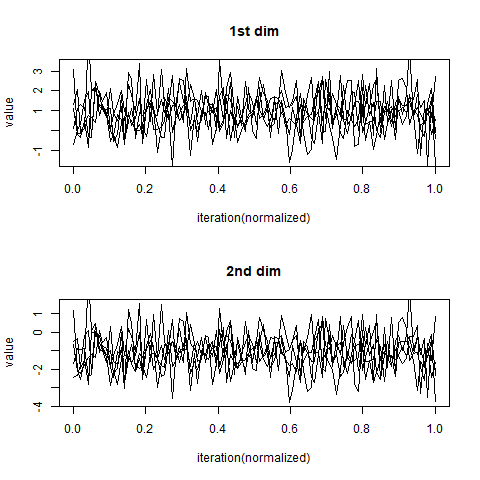
\includegraphics[height=5cm]{prob1_test3_many_process_traceplot.png}
    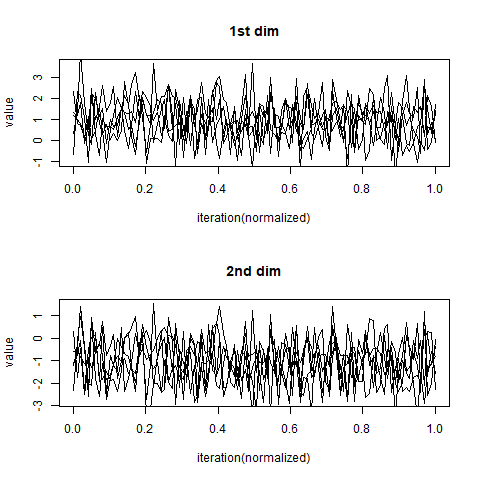
\includegraphics[height=5cm]{prob1_test2_many_process_traceplot.png}
    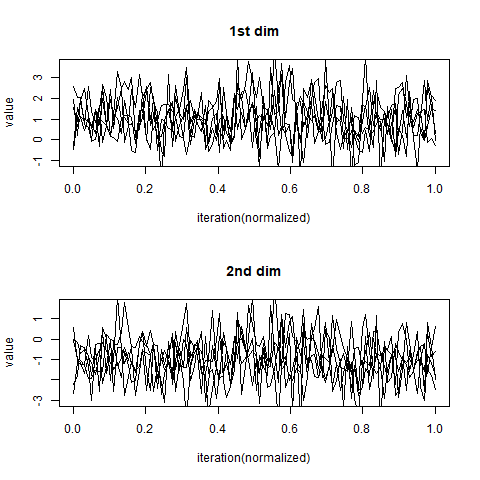
\includegraphics[height=5cm]{prob1_test4_many_process_traceplot.png}
    \caption{left: $\nu=0.1$, middle: $\nu=0.5$, right: $\nu=1$}
\end{figure}


\clearpage
To view more detail, I generate one chain longer for each $\nu$, and construct scatterplot and traceplot.
\begin{figure}[!h]
    \centering
    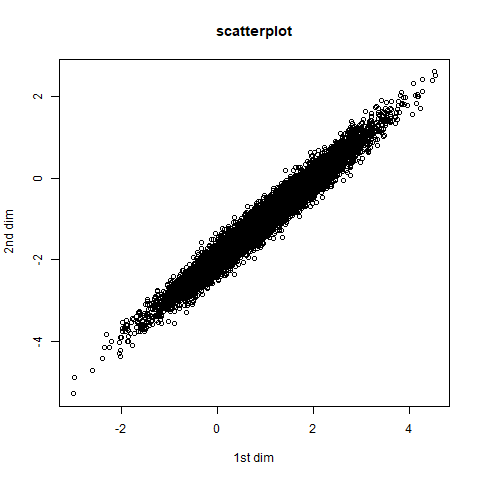
\includegraphics[height=6cm]{prob1_test3_oneprocess_scatter.png}
    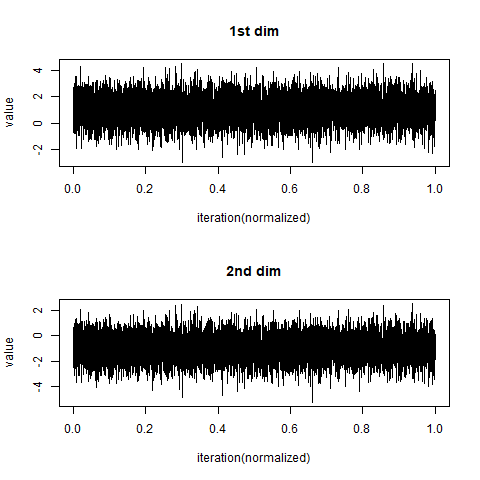
\includegraphics[height=6cm]{prob1_test3_oneprocess_traceplot.png}
    \caption{$\nu=0.1$}
% \end{figure}
% \begin{figure}[hh]
    \centering
    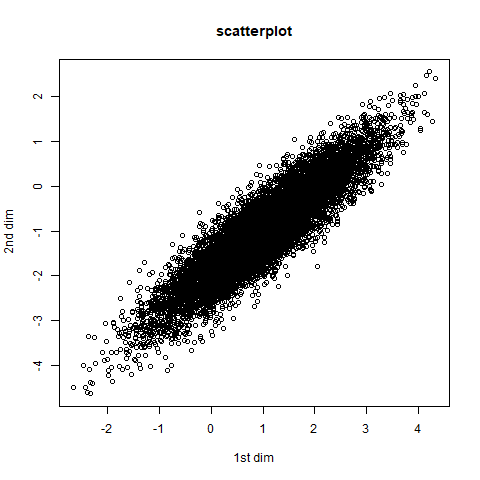
\includegraphics[height=6cm]{prob1_test2_oneprocess_scatter.png}
    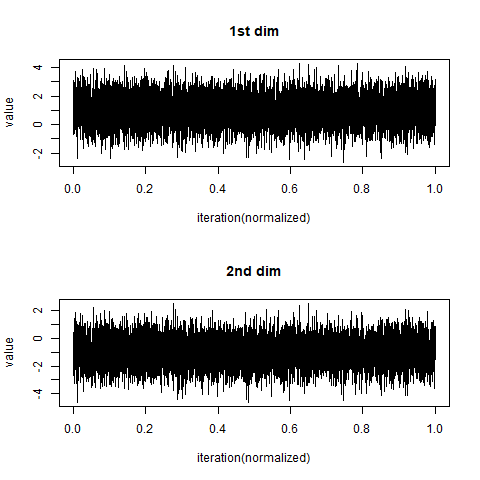
\includegraphics[height=6cm]{prob1_test2_oneprocess_traceplot.png}
    \caption{$\nu=0.5$}
% \end{figure}
% \begin{figure}[hh]
    \centering
    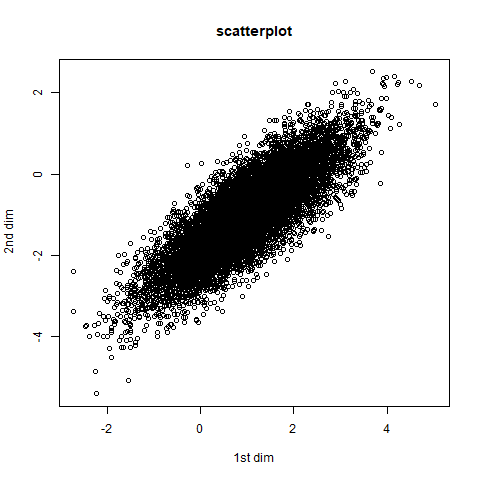
\includegraphics[height=6cm]{prob1_test4_oneprocess_scatter.png}
    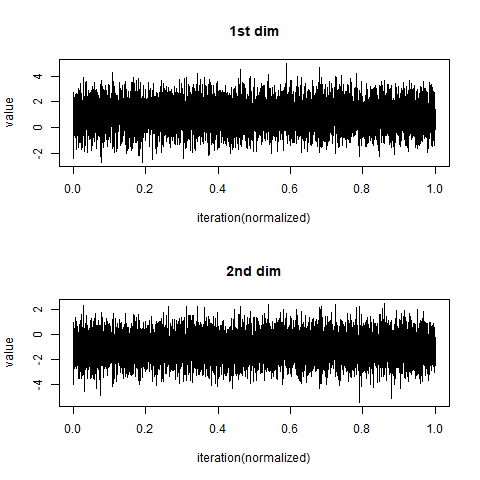
\includegraphics[height=6cm]{prob1_test4_oneprocess_traceplot.png}
    \caption{$\nu=1$}
\end{figure}


The effect of changing $\nu$ are lucidly confirmed by the scatter-plot.
The shapes of scatterplots consist with the calculated covariance matrix above.


\newpage
\section{Problem 2}
\textbf{
The file CAtemps.RData contains two R objects of class SpatialPointsDataFrame, called CAtemp and CAgrid.
CAtemp contains a average temperatures from 1961-1990 at 200 locations (latitude and longitude) in California in degrees Fahrenheit, along with their elevation in meters.
CAgrid contains elevations in meters over a grid of locations.
I've given you some code to get started with this data in HW1.R
}
\textbf{
Consider the following model for the temperature data.
\[Y_i = \mu(s_i;\beta) + e(s_i; \sigma^2, \rho, \tau)\]
where \(\mu(s_i;\beta)=\beta_0+\beta_1 Longitude(s) + \beta_2 Latitude(s)
+\beta_3 Elevation(s)\) and \(e(s_i;\sigma^2,\rho,\tau)\) is a zero mean stationary Gaussian process with
exponential covariance function.
}
\textbf{
Another way of writing this is as
\[Y_i = \mu(s_i;\beta) + Z(s_i; \sigma^2, \rho) + \epsilon_i\]
where now $Z$ is mean zero Gaussian process like $e$ but without the nugget term,
and the $\epsilon$ are iid $N(0,\tau^2)$, independent of Z.
This is important because we want to predict \(\mu(s_i;\beta)+Z(s_i;\sigma^2,\rho)\) without the measurement error.
}


Before solving the main problems, Let's see the data first. Here is average temperature plot of CAtemp.
\begin{figure}[!h]
    \centering
    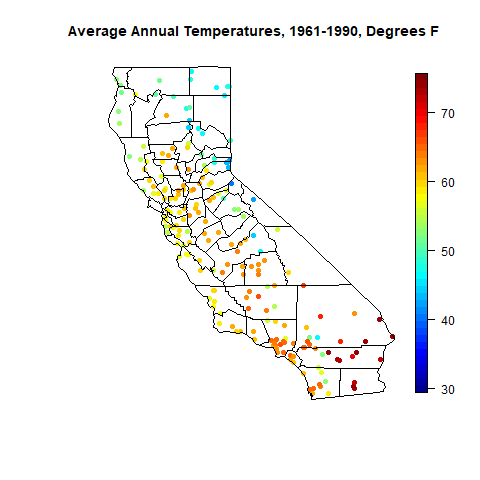
\includegraphics[height=8cm]{prob2_CAtemp_avgtemp.png}
    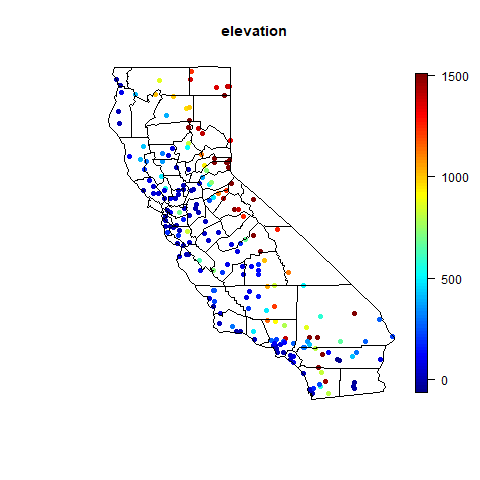
\includegraphics[height=8cm]{prob2_CAtemp_elevation.png}
    \caption{left: average temperature data in CAtemp, right: elevation data in CAtemp}
\end{figure}

We can observe that data points are relatively sparse at upper-right, middle-right and lower-right region.
It may make some problems when we predict the temperature around these region.
And, we can also find something like cluster in the temperature data.
Maybe it need a model concerning with spatial covariance structure to analyze these data.


\clearpage
\subsection{Problem 2-(a)}
\textbf{
Using the CAtemp data, form a preliminary estimate of $\beta$ using ordinary least squares 
and make a color plot of the residuals.
Include your estimates and plot.
}

It is easy work if we use built-in lm function of R.
Load the CAtemps.Rdata and run this code block to get what we want.
\begin{Rcode}
    \begin{verbatim}
ols = lm(avgtemp~lon+lat+elevation, data=CAtemp)
print(ols$coeff) #estimates
CAtemp$ols.residual = ols$residual
    \end{verbatim}
\end{Rcode}
The results of the ordinary least squares' coefficients calculated by R are
\[\hat{\beta}_{0:OLS}=321.5114\]
\[\hat{\beta}_{1:OLS}=2.324105\]
\[\hat{\beta}_{2:OLS}=0.5646805\]
\[\hat{\beta}_{3:OLS}=-0.009648649\]
where \(\mu(s_i;\beta)=\beta_0+\beta_1 Longitude(s) + \beta_2 Latitude(s)+\beta_3 Elevation(s)\).
Be careful to interpret these values. 
They are problematic because they draw from the model without considering a covariance structure.
So, we have better to deal with them only for getting residuals as a step for given spatial model in the problem.


Nextly, the residual at each data point is plotted.
\begin{figure}[!h]
    \centering
    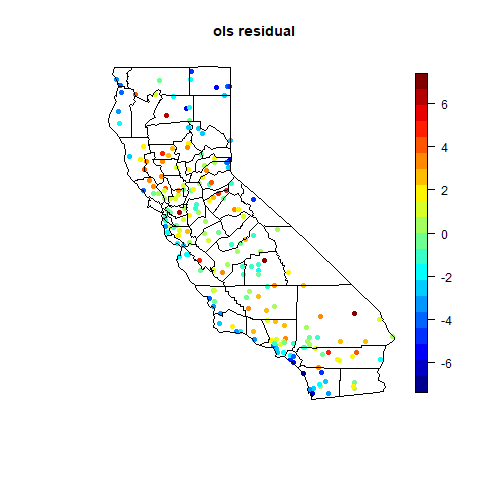
\includegraphics[height=8cm]{prob2_CAtemp_ols_residual.png}
    \caption{the residuals of OLS}
\end{figure}

More once, be careful. 0 is colored by light-green.

We can observe that there are some patterns in residuals. So we have to doubt more that there exists some dependencies.


\clearpage
\subsection{Problem 2-(b)}
\textbf{
Estimate the variogram non-parametrically and then fit the exponential variogram to it using weighted least squares.
Make and include a plot of the nonparametric and parametric variogram functions.
Also store your parameter estimates and report them.
}

For variogram, I use the 'gstat\$variogram' function. Then, the code become (magically) simple.
Here is the key code to get non-parametric variogram. I choose the width to 50.

\begin{Rcode}
    \begin{verbatim}
vg = variogram(ols.residual ~ 1, data = CAtemp, width=50)
print(plot(vg, xlab = "Distance", ylab = "Semi-variogram estimate"))

vgangle = variogram(ols.residual ~ 1, data = CAtemp, alpha = c(0, 45, 90, 135))
print(plot(vgangle, xlab = "Distance", ylab = "Semi-variogram estimate"))
    \end{verbatim}
\end{Rcode}


The variogram plots are here. 
\begin{figure}[!h]
    \centering
    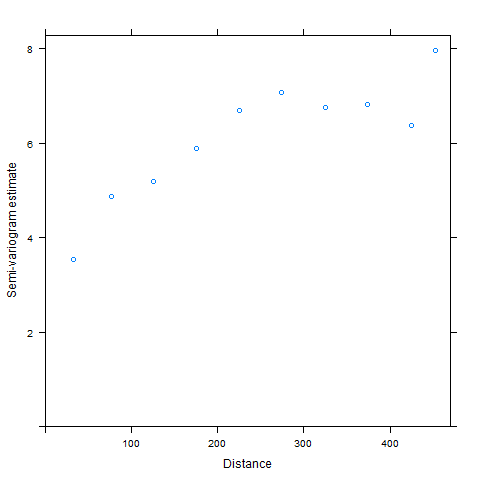
\includegraphics[height=8cm]{prob2_CAtemp_variogram.png}
    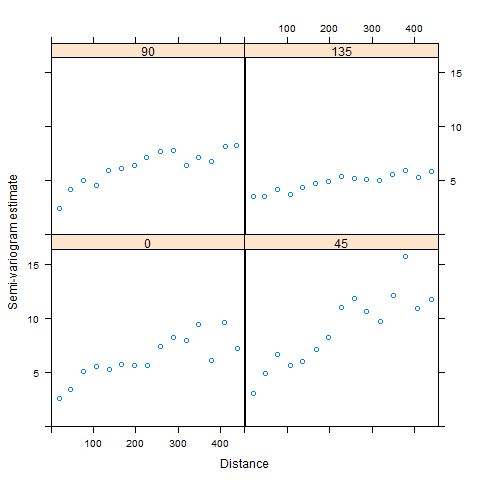
\includegraphics[height=8cm]{prob2_CAtemp_variogram_angle.png}
    \caption{nonparametric variogram fit}
\end{figure}

The brief shape of variogram is not a flat line, so our doubt above is proper as we see here.
And, since the shapes of the rotated variograms have quite similar shapes, this variogram doesn't have a big problem.

Next, I will fit the variogram to exponential variogram model following the direction of the problem.
In this time, the 'gstat\$fit.variogram' funciton make our problem very simple.

\begin{Rcode}
    \begin{verbatim}
# fit
fitvg = fit.variogram(vg, vgm(1, "Exp", range=300, nugget=3)) 

# estimated parameters of variance term
s2.hat = fitvg$psill[2]
rho.hat = fitvg$range[2]
tau2.hat = fitvg$psill[1]
    \end{verbatim}
\end{Rcode}

Below is the result plot.

\begin{figure}[!h]
    \centering
    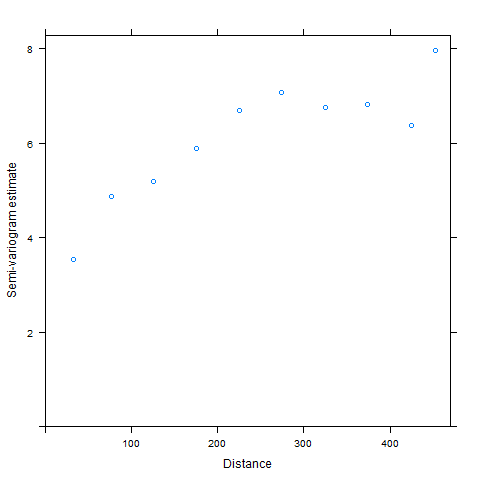
\includegraphics[height=8cm]{prob2_CAtemp_variogram.png}
    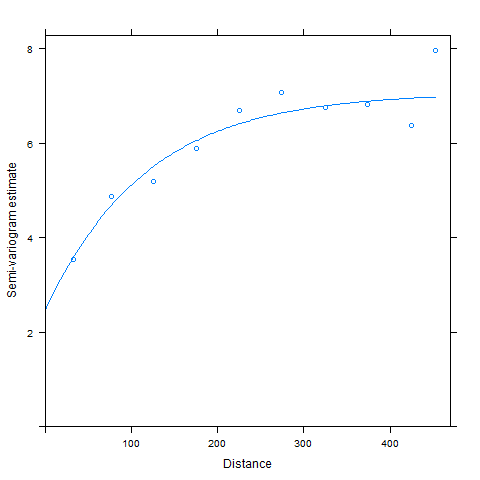
\includegraphics[height=8cm]{prob2_CAtemp_variogram_exp_fit.png}
    \caption{the variogram fitted to the exponential model}
\end{figure}

And, the estimated parameter values of exponential covariance function
calculated by using the least square method are,
(or, using the result of lecture note 1, 48 page's, \(\gamma(h)=C(0)-C(h)=\tau^2+\sigma^2(1-exp(-||h||/\rho))\)),

\[\hat{\sigma}^2 = 4.635655\]
\[\hat{\rho} = 115.7653\]
\[\hat{\tau}^2 = 2.434879\]

So our covariance function becomes, when $i\neq j$
\[C(s_i,s_j)=\sigma^2 exp(-||s_i-s_j||\rho) = 4.635655^2 exp(-115.7653||s_i-s_j||)\]
or when $i=j$,
\[C(s_i,s_j)=\sigma^2 + \tau^2 = 4.635655^2 + 2.434879^2\]


\clearpage
\subsection{Problem 2-(c)}
\textbf{
We will now form the GLS estimate of $\beta$ by hand, rather than using the gls function.
\begin{itemize}
    \item Use the rdist function in fields to create a matrix of distance (in miles) between pairs of locations in CAtemp.
    \item Create the covariance matrix, plugging in your estimates from the fitted variogram. (Hint: Sum tow matrix, one without a nugget and one using the diag function to create the matrix $\tau^2 I$)
    \item Invert the covariance matrix and store it for later reference.
    \item Create the X matrix (Hint: Use cbind.)
    \item Put all the pieces together to form $\hat{\beta}_{GLS}$.
\end{itemize}
}

I implement the procedure GLS by hand. 


Because given data just include the (lat,lon) information, 
I convert from them to miles-measure distance by using the chordal distance.
Then, to get distance matrix, I wse 'rdist' function.
And using it with result of (b)-the estimated covariace function- I make the covariance matrix.
Then, I will invert it and do gls estimation procedure.

Here are the code blocks.


\begin{Rcode}
    \begin{verbatim}
make_chordaldist_u1u2_for_rdist = function(lat, lon){
    mean_earth_radius_in_miles = 3958.8 #by google
    chordaldist_x = mean_earth_radius_in_miles * cos(lat) * cos(lon)
    chordaldist_y = mean_earth_radius_in_miles * cos(lat) * sin(lon)
    chordaldist_z = mean_earth_radius_in_miles * sin(lat)
    chordaldist_mat = cbind(chordaldist_x, chordaldist_y, chordaldist_z)
    return(chordaldist_mat)
}
    
make_EXPcov_mat_without_nugget = function(dist_mat, rho, sigma_sqaure){
    #lecture note 1-2. page 40
    num_row = dim(dist_mat)[1] 
    num_col = dim(dist_mat)[2]
    cov_gamma = matrix(0, num_row, num_col)
    for(i in 1:num_row){
        for(j in 1:num_col){
            cov_gamma[i,j] = exp(-dist_mat[i,j] * rho)
        }
    }
    cov_gamma = cov_gamma * sigma_sqaure
    return(cov_gamma)
}
    
# make distance matrix
CAtemp_data_u1u2= make_chordaldist_u1u2_for_rdist(CAtemp$lat, CAtemp$lon)
CAtemp_data_dist_mat = rdist(CAtemp_data_u1u2, CAtemp_data_u1u2)
# dim(dist_mat) # 200 200
# max(dist_mat)
# min(dist_mat)


# make covariance matrix
CAtemp_data_cov_spatial = make_EXPcov_mat_without_nugget(CAtemp_data_dist_mat, rho.hat, s2.hat)
CAtemp_data_cov_nugget = diag(200) * tau2.hat
CAtemp_data_cov_mat = CAtemp_data_cov_spatial + CAtemp_data_cov_nugget


# gls fit
b0 = rep(1,200)
gls.X = as.matrix(data.frame(b0, CAtemp$lon, CAtemp$lat, CAtemp$elevation))
gls.Y = as.matrix(CAtemp$avgtemp)
CAtemp_data_inv_cov_mat = solve(CAtemp_data_cov_mat)
gls.beta = solve(t(gls.X) %*% CAtemp_data_inv_cov_mat %*% gls.X) %*% 
    t(gls.X) %*% CAtemp_data_inv_cov_mat %*% gls.Y
print("gls coefficients")
cat('(Intercept)    lon       lat    elevation\n',gls.beta,'\n')
print('----------------')
    \end{verbatim}
\end{Rcode}

The results of the GLS' coefficients calculated by R are
\[\hat{\beta}_{0:GLS}=321.5114\]
\[\hat{\beta}_{1:GLS}=2.324105\]
\[\hat{\beta}_{2:GLS}=0.5646805\]
\[\hat{\beta}_{3:GLS}=-0.009647649\]
where \(\mu(s_i;\beta)=\beta_0+\beta_1 Longitude(s) + \beta_2 Latitude(s)+\beta_3 Elevation(s)\).

They are not differ drastically, but maybe OLS model affects more to the standard error of the estimates comparing to OLS model.
And now, since we considered the covariance structure of data,
we can try to interpret the coefficient properly. 
For example, if the elevation increase by a meter, then the temperature decrease about 0.0096 F.
We can do similar interpretation for other coefficients, too.


\clearpage
\subsection{Problem 2-(d)}
\textbf{
Calculate and plot the EBLUP of $\mu+Z$ at the location in CAgrid,
plugging in your estimates from (b) and (c).
Calculate and plot the (estimated) standard error of $Z$ at each prediction location
}

Although the direction of the problem asks for the standard error, 
I will calculate and give the MSE rather than the standard error,
because it shows more interesting things than estimated standard error in this case,
and moreover their roles are similar.

I will re-use the calculated values and my R-functions to get EBLUP and MSE.
Key parts of the code are here.


\begin{Rcode}
    \begin{verbatim}
# make m0(=pred_mu) term(in lec2-2. page38)
pred_X = as.matrix(data.frame(rep(1,664), CAgrid$lon, CAgrid$lat, CAgrid$elevation))
pred_mu = pred_X %*% gls.beta
dim(pred_mu)
head(pred_mu)


# make covariance matrix
#inner
CAgrid_data_u1u2= make_chordaldist_u1u2_for_rdist(CAgrid$lat, CAgrid$lon)
pred_inner_dist_mat = rdist(CAgrid_data_u1u2, CAgrid_data_u1u2)

pred_cov_spatial = make_EXPcov_mat_without_nugget(pred_inner_dist_mat, rho.hat, s2.hat)
# pred_cov_nugget = diag(664) * tau2.hat #no nugget term!
pred_inner_cov_mat = pred_cov_spatial #+ pred_cov_nugget #no nugget term!


#cross
pred_cross_dist_mat = rdist(CAtemp_data_u1u2, CAgrid_data_u1u2)
dim(pred_cross_dist_mat) # 200, 664
pred_cross_cov_mat = make_EXPcov_mat_without_nugget(pred_cross_dist_mat, rho.hat, s2.hat)


## krigging mean
pred_Y = pred_mu + 
    t(pred_cross_cov_mat) %*% CAtemp_data_inv_cov_mat %*% (gls.Y - gls.X%*%gls.beta)
dim(pred_Y)
CAgrid$pred.temp = pred_Y

# sd (I'll skip this. Instead, I'll find mse.)
pred_Y_var_mat = pred_inner_cov_mat - 
    (pred_cross_cov_mat) %*% CAtemp_data_inv_cov_mat %*% pred_cross_cov_mat
# dim(pred_Y_var_mat) #664 664
# pred_Y_var = diag(pred_Y_var_mat)
# CAgrid$pred.sd.temp = sqrt(pred_Y_var)

# predicting mse
cal_b = t(pred_X) - t(gls.X) %*% CAtemp_data_inv_cov_mat %*% pred_cross_cov_mat
pred_mse_mat = pred_Y_var_mat + 
    t(cal_b) %*% solve(t(gls.X) %*% CAtemp_data_inv_cov_mat %*% gls.X) %*% cal_b
pred_mse = diag(pred_mse_mat)
CAgrid$pred.mse.temp = pred_mse
    \end{verbatim}
\end{Rcode}

\clearpage
The result plots of predicted temperature values and MSE values for each location in CAgrid are here.
For convenience of comparison and evaluation, I re-attach original data plots here one more time.
Upper 2 plots are given data, and lower 2 plots are predicted ones from just above works.

\begin{figure}[!h]
    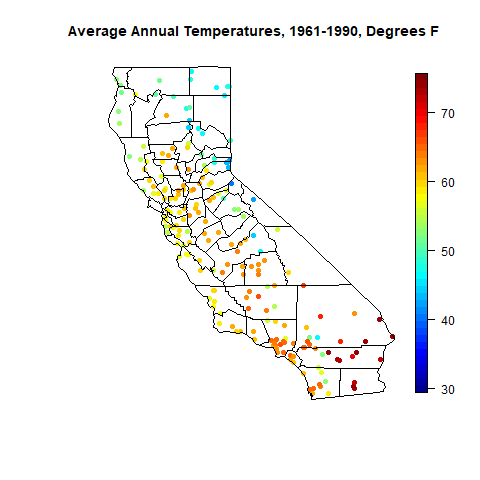
\includegraphics[height=8cm]{prob2_CAtemp_avgtemp.png} 
    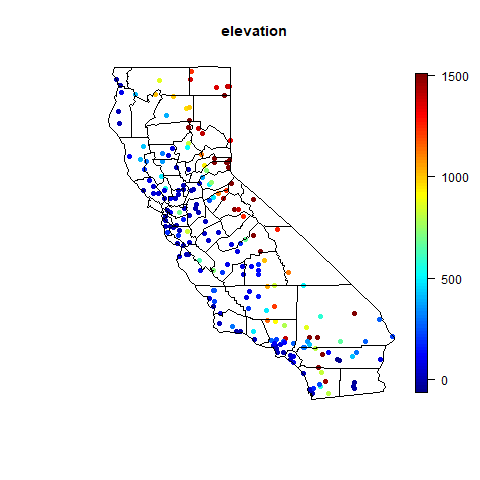
\includegraphics[height=8cm]{prob2_CAtemp_elevation.png} \\
    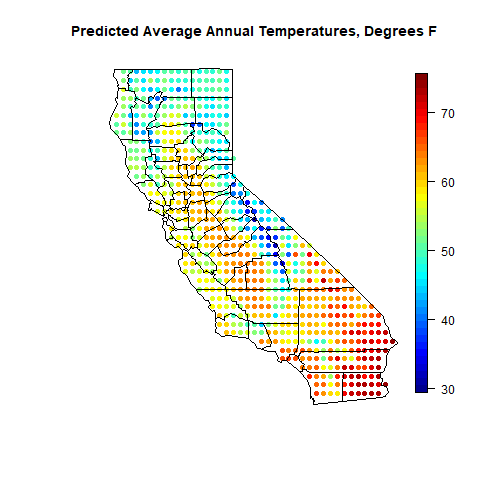
\includegraphics[height=8cm]{prob2_CAgrid_predicted_mean.png}
    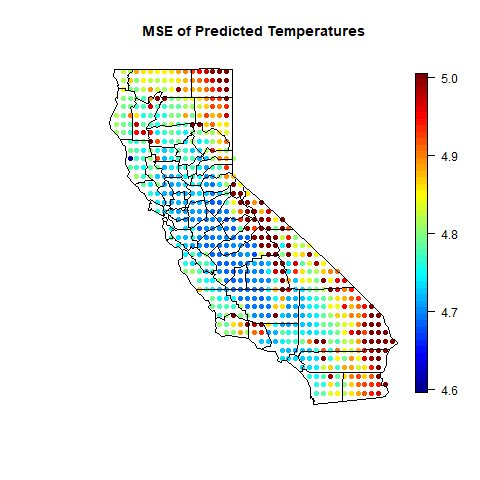
\includegraphics[height=8cm]{prob2_CAgrid_predicted_MSE.png}
    \caption{the temperatures of original data(up-left), the elevations of original data(up-right),
    \\ the predicted temperatures by krigging(down-left), and MSEs by krigging(down-right)}
\end{figure}

We can find that the krigging is quite well enough to predict similar values to original data
at the close krigging points.
And we observe that the elevations matter to the temperature consisting with our common knowledge.
Finally, I should emphasize that the region of sparse data points has relatively higher MSE
than the region of dense data points. It is reasonable.

\end{document}